%%%%%%%%%%%%%%%%%%%%%%%%%%%%%%%%%%%%%%%%%
% "ModernCV" CV and Cover Letter
% LaTeX Template
% Version 1.11 (19/6/14)
%%%%%%%%%%%%%%%%%%%%%%%%%%%%%%%%%%%

%----------------------------------------------------------------------------------------
%	PACKAGES AND OTHER DOCUMENT CONFIGURATIONS
%----------------------------------------------------------------------------------------

\documentclass[11pt,a4paper,sans]{moderncv} % Font sizes: 10, 11, or 12; paper sizes: a4paper, letterpaper, a5paper, legalpaper, executivepaper or landscape; font families: sans or roman

\moderncvstyle{classic} % CV theme - options include: 'casual' (default), 'classic', 'oldstyle' and 'banking'
\moderncvcolor{blue} % CV color - options include: 'blue' (default), 'orange', 'green', 'red', 'purple', 'grey' and 'black'
%\usepackage{vntex} % If you wanna type vietnamese sytle
%\usepackage[utf8]{inputenc}
\usepackage[english]{babel}
\usepackage{graphicx}
%\usepackage[vietnam,english]{babel}
\usepackage{lipsum} % Used for inserting dummy 'Lorem ipsum' text into the template


%\usepackage{url}


\usepackage[scale=0.85]{geometry} % Reduce document margins
%\setlength{\hintscolumnwidth}{3cm} % Uncomment to change the width of the dates column
%\setlength{\makecvtitlenamewidth}{10cm} % For the 'classic' style, uncomment to adjust the width of the space allocated to your name

%----------------------------------------------------------------------------------------
%	NAME AND CONTACT INFORMATION SECTION
%----------------------------------------------------------------------------------------

\firstname{Sony} % Your first name
\familyname{Huynh} % Your last name

% All information in this block is optional, comment out any lines you don't need
\title{Curriculum Vitae}
\address{65/27A Phu Tho}{Ward 1, District 11, Ho Chi Minh City}
\mobile{+84 933826695}
\email{hpsony94@gmail.com}
\homepage{linkedin.com/in/hpsony}{linkedin.com/in/hpsony}
\extrainfo{Skype, Whatapps, Facebook, Github: @hpsony94}
\photo[100pt][0.8pt]{avatar} % The first bracket is the picture height, the second is the thickness of the frame around the picture (0pt for no frame)
\quote{"A person who never made a mistake never tried anything new"}

%----------------------------------------------------------------------------------------

\begin{document}

\makecvtitle % Print the CV title

\section{PERSONAL DETAILS}
\cvitem{}{Full name: Huynh Pham Sony}
\cvitem{}{Date of birth: July $20^{th}$, 1994.} 
%\cvitem{Objective}{After graduate I am going to looking for the national company in IT field, to study more and gain the experience that I need, what is missing.
%A dedicated worker aiming to help achieve company goals and take on more responsibility as quickly as possible.%
%}

%----------------------------------------------------------------------------------------
%	EDUCATION SECTION
%----------------------------------------------------------------------------------------

\section{EDUCATION BACKGROUND}

\subsection{\textbf{Ho Chi Minh city University of Technology}}

\cvitem{2012--2017}{\textbf{Computer Engineering}}
\cvitem{}{The Honor Program at Faculty of Computer Science and Engineering.}
\cvitem{\textbf{GPA}}{\textbf{8.21/10.}}

%----------------------------------------------------------------------------------------
% SKILL SECTION
%----------------------------------------------------------------------------------------

\section{SKILLS} 

\subsection{Technical Skills}

{\color{black} {\cvitem{Languages}{ C++/C, Verilog HDL, JavaScript, Visual Basic, TTCN3, \LaTeX.}}} 
{\color{black} {\cvitem{Environment}{Linux(SUSE, Ubuntu) \& Windows.}}} 
%Photoshop, \LaTeX, 
{\color{black} {\cvitem{\textbf{Advanced field}}{Embedded system, Internet of Things, Networking, Telecommunications.}} }

\cvitem{\textbf{OpenSource experience}}{OPENSAF, ASTERISK(*).}

\subsection{Personal Skills}
{\color{black} {\cvitem{Leadership}{\fontsize{20}{20}\selectfont $\bullet \bullet \bullet \bullet \circ  $}}}
{\color{black} {\cvitem{Planning}{\fontsize{20}{20}\selectfont $\bullet \bullet \bullet  \bullet \circ  $}}}
{\color{black} {\cvitem{Creativity}{\fontsize{20}{20}\selectfont $\bullet \bullet \bullet \circ    \circ  $}}}
\cvitem{\textbf{English}}{Good communication skills.}
\cvitem{}{Have much experience in reading technical books, writing an email.}
\cvitem{}{Join the Bible club in English.}

%----------------------------------------------------------------------------------------
%	COMMUNICATION SKILLS SECTION
%----------------------------------------------------------------------------------------
\newpage

\section{\textbf{WORKING EXPERIENCE}}
\subsection{Ho Chi Minh city University of Technology}
\cvitem{May 2014}{Designed Single Cycle CPU with Hardware description languages On DE2 Board.}
\cvitem{Dec 2014}{"Smart Led Matrix" - Show the notification of smartphone on led devices.}
\cvitem{Oct 2015}{"Retro game" on DE2 Board and 89V51 KIT with C \& Verilog HDL language.}
\cvitem{Oct 2015}{"Snack game" on 89V51 KIT with C language.}
\cvitem{Nov 2015}{"Car Racing" on DE2 Board with Verilog HDL language.}
\cvitem{Feb 2016}{"sJob Android Application" - Help students find out part-time jobs..}
\cvitem{2015--2016}{Joined scientific researches students with the topic \textbf{"Vietnamese Speech Recognition".}}
\cvitem{}{Base on ISD9160 chipset, we had time to study and create new model for supporting to recognize Vietnamese speech.}
\cvitem{}{We used Trello board to manage all the tasks during those times, and reported the state of tasks every single sprint (2 weeks)}
\cvitem{2016-2017}{\textbf{Graduation Thesis} - "Investigation and Implementation of a vehicle emissions monitoring system"}
\cvitem{}{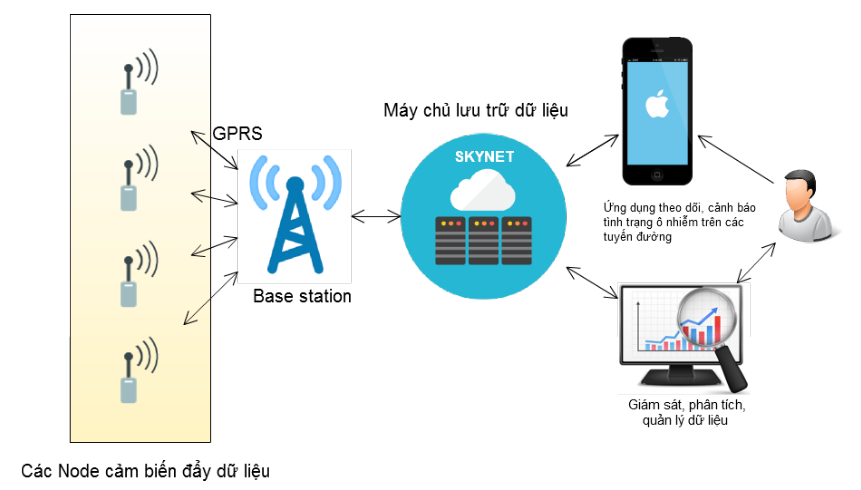
\includegraphics[scale=0.45]{thesis}}
\cvitem{}{As the environment and traffic situations nowadays, the needs of information about those two are very important but limited the supplier. Therefore, we studied and made this project about the system of collecting environment elements as well as traffic data by sensor nodes. Thanks to the explosive development of Internet of Things and based on knowledge about the linking between quality of environment and elements.}
\cvitem{}{We built the entirely new system which featuring a new sensor node that can operate without the main power grid and can resist the harsh weather conditions like extremely sunny or heavy raining. Moreover, we provided the friendly website and mobile app to user as well as useful APIs for third party developer.}

\subsection{DEK TECHNOLOGIES PTY. LTD}
\cvitem{6-8/2016}{\textbf{Software Engineer Internship Summer 2016}}
\cvitem{}{The project is to deploy High Availability for persistent chat service by using \href{https://sourceforge.net/p/opensaf/wiki/Home/}{\textbf{OPENSAF}.}}
\cvitem{}{We have done High Availability for Chat service and Chat application by using OPENSAF, C++, and Framework Qt.}

\newpage
\cvitem{Oct 2016 - Sep 2017}{\textbf{Software Engineer in IMTAF (IMS Testing Automation Framework)}}
\cvitem{}{Experience in field with protocols: TCP/UDP, IP, SIP, SDP, DIAMETER, RTP, MEGACO/H.248.}
\cvitem{}{Work using Agile Software Development with Hansoft and performing code reviews in Gerrit and ClearCase.}
\cvitem{}{Experience with various IMS nodes: CSCF, HSS, SBG, MTAS and various Ericsson IMS features. Test automation in integration with Jenkins.}
\cvitem{}{Automated network level testing of the new features after integration. It involves development of automated test suite for testing the new as well as legacy features. The scope is to automate the test cases and prepare a test suite.}
\cvitem{}{Main activities: implement new change request and test cases in TTCN-3 language. Execute, perform regression test, analyze test reports and release the framework every single sprint.}

\cvitem{9-11/2017}{\textbf{Consultant Software Engineer at Ericsson AB}}
\cvitem{}{I had an golden opportunity to work with my partners in Ericsson Office for 2 months in Stockholm, Sweden.}

\cvitem{Nov 2017 - Present}{\textbf{Software Engineer in IMS Network Feature Test}}
\cvitem{}{Developing of Automating System Test and Feature Test of Ericsson's Enterprise Communication solution on a system and network integration test level, using Java, Bash and TTCN3 languages. Continuous integration with Jenkins, deployment with Docker.}
\cvitem{}{- IMS architecture and components}
\cvitem{}{- IMS core nodes MTAS, CSCF, SBG, HSS, MGC, DNS, CUDB.}
\cvitem{}{- Verification and Troubleshooting of IMS E2E functionalities}
\cvitem{}{- INT test suites based on  IMS Test Automation Framework developing and maintanance}
\cvitem{}{- SIP, SDP, RTP, Diameter, DNS, TCP/IP, IP technologies}
\cvitem{}{- Linux knowledge: file system and bash scripting}
\cvitem{}{Working in an agile team using ScrumWorks, Open ALM and Git/Gerrit. Actively taking part in planning sprints and participating in retrospective meetings.}

\newpage
\subsection{PERSONAL PROJECT}
\cvitem{July 2017 - Present}{\textbf{Auto Dialer Service}}

\cvitem{}{Auto Dialer Service is an API application written in NodeJS for \href{https://www.asterisk.org/}{\textbf{Asterisk}} to send voice broadcasts. It can generate multiple simultaneous calls to a list of numbers and play a custom audio message. Auto Dialer Service can receive DTMF input options and connect to any predefined destinations. We can find different occasions where Auto Dialer Service can solve problems with minimum effort like event management, customer relations, staff management and where ever people like to hear from you. Auto Dialer Service is simple in design and user interface so that anyone can install and start call blasting within few minutes via providered API.}
\cvitem{}{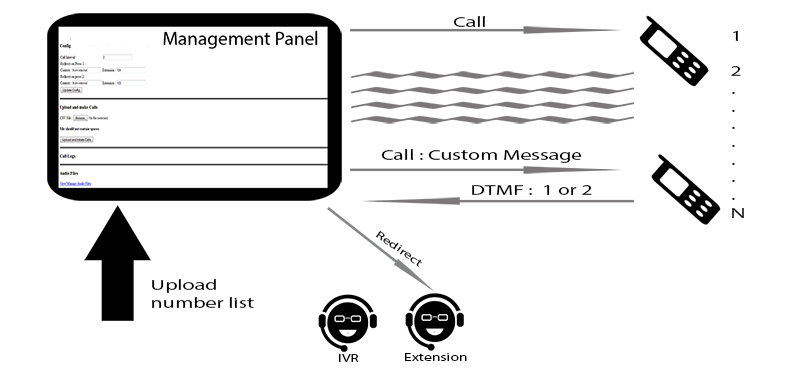
\includegraphics[scale=0.55]{autodial}}
\cvitem{}{Key Features:}
\cvitem{}{- Supports multiple simultaneous calls to a list of numbers.}
\cvitem{}{- Possibility of separate audio messages for each number.}
\cvitem{}{- Configurable redirect destinations to any asterisk context and extension (external or internal number,ring groups,queue,ivr etc)..}
\cvitem{}{- Dialing Screen displays call status and DTMF response via Web App.}
\cvitem{}{- Detailed call log with call deposition and DTMF received.}
\cvitem{}{- Uses regular outbound routing for broadcast,use any trunk or dialpattern.}

\section{EXPERIENCE \& SOCIAL ACTIVITIES}

\cvitem{2012--2015}{Operating and organizing social events for high school.}
\cvitem{2012--2013}{Joined the voluntary activities of WINBK team in University.}
\cvitem{2013--2014}{Joined the "TIEP SUC MUA THI - BACH KHOA 2013" voluntary activities in the summer term.}
\cvitem{2013--2014}{Management and administration of the forum svdhbk.com.}
\cvitem{2014}{Technical Head of "RUNG CHUONG VANG 2014" academic program organized by my faculty .}
\cvitem{2014--2016}{Leader of Fellowship of evangelical students from my university.}
%\cvitem{2013--Present}{Sale second-hand smart phones via online visit at \textit{\textbf{fb.com/hpsonyshop}}. }
\cvitem{2015--Present}{Leader of Bach Khoa Toan Free ref to \href{http://bkfree.info}{\textit{\textbf{bkfree.info}.}}}

%----------------------------------------------------------------------------------------
%	INTERESTS SECTION
%----------------------------------------------------------------------------------------

\newpage

\section{ACHIEVEMENT} 
\cvitem{Special Prize}{\textbf{Global IT Startup Contest Vietnam 2015} from Handong Global University}
\cvitem{}{Team's product is "Smart Neck-pillow".}
\cvitem{Hard work}{\textbf{Hackathon Contest 2016} from ATWARE corporation}
\cvitem{}{Team's product is "AGILES".}

\cvitem{Dec 2016}{\textbf{Student Award - "Sinh vien 5 tot"} of Ho Chi Minh city}
\cvitem{}{Vietnam National Union of Students}

\subsection{Certificate}
\cvitem{March 2016}{ IBM Bluemix Certificate - Apply Bluemix technology applications for IoT System.}


\section{REFERENCES}


\cvitem{}{\href{https://www.youtube.com/playlist?list=PL8jT36S3YC5x2csTofRDTdygF2-bZizm0}{https://www.youtube.com/playlist?list=PL8jT36S3YC5x2csTofRDTdygF2-bZizm0}}
\cvitem{}{\textbf{Dr. Pham Hoang Anh}, Lecturer in Ho Chi Minh City University Of Technology}
\cvitem{}{Email: anhpham@hcmut.edu.vn - Phone: (+84) 967 333 820}

\section{INTERESTS}


\cvlistdoubleitem{Volleyball}{Designing}
\cvlistdoubleitem{Music}{Guitar}
\cvlistdoubleitem{Running}{Learning}

%----------------------------------------------------------------------------------------
%	COVER LETTER
%----------------------------------------------------------------------------------------


\end{document}
